\documentclass[]{scrartcl}
\title{Vorlesung Analysis II}
\usepackage{amsmath,amssymb,amsfonts}
\usepackage{stmaryrd}
\usepackage{mathtools}
\usepackage{latexsym}
\usepackage{graphicx}
\usepackage{tikz}
\usepackage{xcolor}
\usepackage{soul}
\usepackage{hyperref}
\usepackage{tipa}
\usepackage[dvipsnames]{xcolor}
\hypersetup{
	colorlinks=true,
	linkcolor=blue,
	filecolor=magenta,      
	urlcolor=cyan,
	pdftitle={Overleaf Example},
	pdfpagemode=FullScreen,
}
\newcommand{\redcircle}[1]{%
	\tikz[baseline=(char.base)]{
		\node[shape=circle, draw=red, text=red, thick, inner sep=1pt] (char) 
		{\textbf{#1}};
	}%
}
\setul{1pt}{3pt} % Linienhöhe und Abstand zum Text (optional anpassbar)

\setlength{\topmargin}{-.5in} \setlength{\textheight}{9.25in}
\setlength{\oddsidemargin}{0in} \setlength{\textwidth}{6.8in}
\setlength{\parindent}{0pt}

\begin{document}
	\textbf{\underline{Teil 1: Differentialgleichung im $\mathbb{R}^n$}}\\
	\\
	\textbf{\underline{an4: Mehrdimensionales Ableiten}}\\
	\\
	\textbf{\underline{\underline{Stichworte:} Richtungsableitung, partielle Ableitung, totale Ableitung, Klein-o}}\\
	\\
	\textbf{\underline{Literatur:}} \setulcolor{blue}\ul{[Hoff], Kapitel 9.4}\\
	\\
	\textbf{4.1. \underline{Einleitung:}} Wir führen den Differenzierbarkeitsbegriff  für Funktionen $\mathbb{R}^n\rightarrow\mathbb{R}^m$ ein: über Richtungableitungen entlang der Koordinatenachsen gelangen wir zu partiellen Ableitungen. Wir definieren die totale Ableitung und sehen wie mit den partiellen Ableitungen der Komponentenfunktionen berechnet werdeb kann. Die "Linearsierung" von f ergibt also die Matrix $Df(a)\in\mathbb{R}^{m x n}$ so, dass $f(x) \approx f(a)+Df(a)\cdot(x-a)$ in gute Mäherung ist.\\
	\\
	\textbf{4.2 \underline{Konvention:}} Betrachte Funktionen $f:U\rightarrow\mathbb{R}^m$ mit $U \subseteq \mathbb{R}^n$.\\
	Sei $a \in U$ ein \setulcolor{orange}\ul{innerer Punkt} von U, d.h. $\exists S > 0: U_a^s\subseteq U.$\\
	Man könnte D füt die Definitionsmenge von f schreiben, tun dies aber wegen Verwechslungsgefahr mit den anderen D's in diesen Kapitel nicht.\\
	\\
	\textbf{4.3.} Hatten: im Fall \underline{n=m=1} ist $f'(a)=\lim_{x\rightarrow a}\frac{f(x)-f(a)}{x-a}$ die Ableitung.  ($\mathbb{R}\supseteq U \ni x \rightarrow a$)\\
	\\
	\textbf{4.4.} \underline{Falls $n>1$}, ist x-a ein Vektor und der Differentialquotient nicht bildbar.\\
	\\
	\textbf{4.5.} \underline{Falls n=1, $m\geq 1$}, ist $\frac{1}{x-a} \cdot (f(x)-f(a))$ der (n-dimensionale) Differenzenquotient \underline{$\in \mathbb{R}^m$},\\
	und \setulcolor{yellow} \ul{Df(a)}:=\setulcolor{red}\ul{$\lim_{x\rightarrow a}\frac{f(x)-f(a)}{x-a}$ die Ableitung}. $(\mathbb{R}\supseteq U \ni x \rightarrow a)$\\
	\begin{figure}[h]
		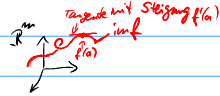
\includegraphics[width=7 cm,height=3cm]{bsp kap 4.5}
	\end{figure}\\
	Sind $f_1,...,f_m$ die Komponentenfunktionen von f, d.h. $f(x)=\begin{pmatrix}
		f_1(x)\\ \vdots \\f_m
	\end{pmatrix}$ für alle x $\in$\underline{$U\subseteq\mathbb{R}$},\\
	also die $f_i:U\rightarrow\mathbb{R}, f_i:=pr_i \circ f$, so ist\\
	\begin{equation}
		\frac{1}{x-a}\cdot(f(x)-f(a))=\frac{1}{x-a}\cdot\begin{pmatrix}
			f_1(x)-f_1(a)\\ \vdots \\ f_m(x)-f_m(a)
		\end{pmatrix} \xrightarrow{x\rightarrow a}\begin{pmatrix}
		f_1'(a)\\ \vdots \\ f_m'(a)
		\end{pmatrix},
	\end{equation}\\
	falls alle Komponentenfunktionen $f_i$ diffbar in a sind.\\
	Wir erhalten $Df(a)=\begin{pmatrix}
		f_1'(a)\\ \vdots \\f_m'(a)
	\end{pmatrix} \in \mathbb{R}^m$ in diesem Fall und schreiben auch \setulcolor{yellow} \ul{f'(a)} für Df(a).\\
	\\
	\textbf{4.6 \underline{Bsp.:}} Betrachten $f:\mathbb{R}\rightarrow\mathbb{R}^2, f(x):=\begin{pmatrix}
		x\\x^2
	\end{pmatrix}.$ also :$f_1(x)=x, f_2(x)=x^2, f_1'(x)=1, f_2(x)=2x$, wir erhalten f'(a)=$\begin{pmatrix}
		f_1'(a)\\f_2'(a)
	\end{pmatrix}=\begin{pmatrix}
	1\\2a
	\end{pmatrix}$ für $a\in \mathbb{R}$.\\
	\\
	\textbf{4.7 \underline{Fall n $>$1:}} Mit $a \in U\subseteq \mathbb{R}^n$ und der Konvention, dass a ein innerer Punkt von U ist, können wir und mit $x \in U$ aus verschiedenen Richtungen an a annähern, Ist etwa $v\in \mathbb{R}^n\backslash\{0\}$ ein Vektor, der uns die "Richtung" der Ableitung angeben soll, so wollen wir f "in diese Richtung" ableiten, d.h. die Funktion \setulcolor{yellow} \ul{$f_v$:}$\begin{cases}
		]-s,s[\rightarrow \mathbb{R}^m\\
		t\rightarrowtail f(a+tv)
	\end{cases}$\\ 
	in $(t_0=)0$ ableiten, und haben die Fragestellung auf \setulcolor{blue}\ul{4.5} zurückgeführt. Dabei ist s\textgreater0 geeignet so, dass $U_a^{s||v||}\subseteq U$ ist (damit auch a$\pm s v \in U$ ist). Hier ist es üblich, den Richtungsvektor auf 1 zu \underline{normieren}, d.h. $||v||=1$ vorauszusetzen, damit wir in der Bedingung an s einfach $U_a^s \subseteq U$ schreiben können.\\
	\\
	\textbf{4.8 \underline{Def.:}} Das Ergebnis \setulcolor{yellow}\ul{$D_v f(a)$}:=$\lim_{t\rightarrow 0}\frac{1}{t}\cdot(f(a+tv)-f(a))\in\mathbb{R}^m$, d.h. \setulcolor{red}\ul{$D_v f(a):=f_v'(0)$}, heißt \ul{Richtungsableitung von f in a in Richtung v}.\\
	Diese beschreibt also das Wachstum von f entlang der Geraden $g:\mathbb{R}\rightarrow \mathbb{R}^n$ \\
	g(t):=a+tv (in Parameterform mit $t \in \mathbb{R}$ als Parameter).\\
	\\
	\textbf{4.9 \underline{Bsp.:}}$\bullet f: \mathbb{R}^2 \rightarrow\mathbb{R}^3, \begin{pmatrix}
		x\\y
	\end{pmatrix}\rightarrowtail \begin{pmatrix}
	x+y\\x-y\\2x^2
	\end{pmatrix}$ soll in $a=\begin{pmatrix}
	-3\\4
	\end{pmatrix}$ abgeleitet werden, und zwar \underline{entlang} $v=\begin{pmatrix}
	1\\1
	\end{pmatrix}$ (es sei $||\cdot||=||\cdot||_\infty$).\\
	dazu bilden wir $f_v: t\rightarrowtail f(a+tv)= f \begin{pmatrix}
		-3+t\\4+t
	\end{pmatrix}=\begin{pmatrix}
	1+2t\\-7\\2(-3+t)^2
	\end{pmatrix}=\begin{pmatrix}
	f_{v,1}(t)\\f_{v,2}(t)\\f_{v,3}(t)
	\end{pmatrix}, 
	\begin{cases}
	f_{v,1}(t)=2\\f_{v,2}(t)=0\\f_{v,3}(t)=4(-3+t)
	\end{cases}$\\
	deren Ableitung ist\\
	$D_{\begin{pmatrix}
		1\\1
	\end{pmatrix}} f\begin{pmatrix}
	-3\\4
	\end{pmatrix}'(0)=\begin{pmatrix}
	2\\0\\4\cdot(-3+0)
	\end{pmatrix}=\begin{pmatrix}
	2\\0\\-7
	\end{pmatrix}$.\\
	$\bullet$ Dasselbe f soll entlang der Koordinatenachsen $v_1=\begin{pmatrix}
		\textcolor{red}{1}\\\textcolor{red}{0}
	\end{pmatrix}=: e_1$ und $v_2 =\begin{pmatrix}
		\textcolor{cyan}{0}\\\textcolor{cyan}{1}
	\end{pmatrix}=:e_2$ in $ a= \begin{pmatrix}
		-3\\4
	\end{pmatrix}$ abgeleitet werden. haben $f_{e_1}:t \rightarrowtail f(a+t e_1)=f\begin{pmatrix}
		-3+t\cdot\textcolor{red}{1}\\4+t\cdot\textcolor{red}{0}
	\end{pmatrix}=\begin{pmatrix}
		1+t\\-7+t\\2(-3+t)^2
	\end{pmatrix}\leadsto\begin{cases}
	f_{e_1,1}(t)=1\\f_{e_2,2}(t)=1\\f_{e_3,3}(t)=4(-3+t)
	\end{cases}$\\
	mit Abl. \underline{\underline{$D_{e_1}f\begin{cases}
				-3\\4
			\end{cases}$}}=$f_{\begin{pmatrix}
		1\\0
	\end{pmatrix}}'(0)=\begin{pmatrix}
	1\\1\\-12
	\end{pmatrix},$\\
	und mit $f_{e_2}: t\rightarrowtail f(a+t e_2)=f\begin{pmatrix}
		-3t\cdot\textcolor{cyan}{0}\\4+t\cdot\textcolor{cyan}{1}
	\end{pmatrix}=\begin{pmatrix}
		1+t\\-7-t\\18
	\end{pmatrix}\leadsto\begin{cases}
	f_{e_2,1}(t)=1\\f_{e_2,2}(t)=1\\f_{e_2,3}(t)=4(-3+t)
	\end{cases}$\\SCHAU NACH WAS HIER RICHTIG IST E 2 ODER E 1-3!!!!!!!!!!\\
	mit Ableitung \underline{\underline{$D_{e_1}f\begin{cases}
			-3\\4
		\end{cases}$}}=$f_{\begin{pmatrix}
		0\\1
		\end{pmatrix}}'(0)=\begin{pmatrix}
	1\\1\\0
	\end{pmatrix}$.\\
	\\
	\textbf{4.10 \underline{Def.:}} Für $j\in\{1,...,n\}$ heißt die Richtungsableitung \setulcolor{yellow} \ul{$D_jf(a)=\frac{\delta f}{\delta x_j}$}:=\setulcolor{red}\ul{$D_{e_j}f(a)$} $\in \mathbb{R}^m$\\
	von f in a in Richtung des j-ten Kanonischen Einheitsvektors $e_j = (0,...,0,\textcolor{cyan}{1}(\text{setlle j}),0,...,0)\in\mathbb{R}^n\\$
	(d.h. in richtung der j-ten Koordinatenachse)\\
	dir \setulcolor{red}\ul{j-te partielle ableitung von f in a}.\\
	\\
	\textbf{4.11 \underline{Bem.:}}$\bullet$ Für m=1 erhält man dies Ableitung $\in \mathbb{R}$ durch Ableiten nach der j-ten Variable, denn 
	\begin{align}
		D_{\textcolor{cyan}{e_j}}f(a)&= \lim\limits_{t\rightarrow 0}\frac{1}{t}(f(a+t\textcolor{cyan}{e_j})-f(a))\\
		&=\lim\limits_{t\rightarrow0}\frac{1}{t}\cdot(f(...,a_{j-1},a_j+t\cdot\textcolor{cyan}{1}, a_{j+1},...)-f(...,a_{j-1},a_j,a_{j+1},...)),
	\end{align} \\
	\\
	\textbf{4.12 \underline{Bsp.:}}
	
	
	
\end{document} 